\chapter{Dodatek}
\label{cha:dodatek}

\section{Opis plików}
Wszystkie pliki utworzone podczas pracy nad projektem zostały wysłane razem ze sprawozdaniem oraz są dostępne pod adresem \url{http://github.com/Kyhu/wsw-neuro}, gdzie mogą być w dalszym ciągu aktualizowane. Poniżej krótko opisano strukturę projektu.

\begin{figure}[tbph!]
\centering
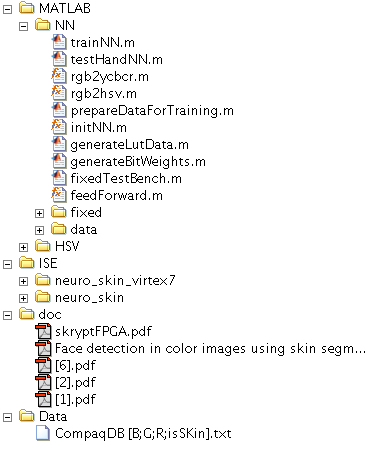
\includegraphics[width=0.63\linewidth]{images/tree.png}
\caption{Struktura katalogów}
\label{fig:tree}
\end{figure}

\begin{itemize}
\item MATLAB - folder zawierający wszystkie utworzone pliki środowiska MATLAB.
\subitem NN
\subsubitem trainNN.m - skrypt trenujący model sieci neuronowej.
\subsubitem testHandNN.m - skrypt testujący sieć na przykładowym obrazie.
\subsubitem generateLutData.m - skrypt generujący dane dla LUTa w module języka verilog.
\subsubitem generateBitWeights.m - skrypt generujący linijki kodu veriloga odpowiadające za przechowywanie wartości wag sieci neuronowych.
\subsubitem fixedTestBench - test bench dla skryptów feedForward oraz fix\_feedforward.
\subsubitem feedForward.m - funkcja symulująca moduł neural\_networks.v na liczbach zmiennoprzecinkowych
\subsubitem fix\_feedForward.m - funkcja symulująca moduł neura\_networks.v na liczbach stałoprzecinkowych
\subsubitem data - folder zawierający zapisane modele sieci Neuronowych (wagi) oraz testowe obrazy.
\subitem HSV - folder zawierający skrypty wykorzystane do testowania modułu rgb2hsv zaimplementowanego w veriolgu.
\item ISE - folder zawierający projekty realizowane w środowisku ISE.
\subitem neuro\_skin - projekt finalny realizowany na kartę Spartan-6.
\subitem neuro\_skin\_virtex7 - projekt finalny przerzucony na tor wizyjny karty virtex7 (z projektu pbas)
\item doc - folder zawierający wykorzystane artykuły naukowe. Artykuł dostarczony przez prowadzącego jest opisany pełnym tytułem, pozostałe są oznaczone odnosząc się do jego bibliografii.
\item Data - folder zawierający bazę danych wykorzystaną do trenowania sieci neuronowej. (Compaq Database - \url{https://archive.ics.uci.edu/ml/machine-learning-databases/00229/Skin_NonSkin.txt})
\end{itemize}